\chapter{The Standard Model of Particle Physics \label{chapter2_theory}}

Four fundamental forces are known up to know: the electromagnetic force, the weak force, the strong force and the gravitational
force. The first three forces are well described within the SM, while the latter can be described by general relativity.
For all these interactions, except of the gravitational force, an unique quantum field theory is existing. The interactions are
mediated by gauge bosons. The SM in its full magnificence is represented by a gauge group of the form $\mathrm{SU}(3)_C\times\mathrm{SU}(2)_L\times\mathrm{U}(1)_Y$,
where the indices correspond to the color charge $C$, the weak isospin $L$ and the weak hypercharge $Y$. The $\mathrm{SU}(3)_C$ gauge group
describes the quantum chromodynamics (QCD), which force (strong force) couples to three color charges (red, green or blue). Demanding
local gauge symmetry within the QCD lagrangian 8 gauge bosons are predicted for the strong force, namely gluons with different color charge.
The weak and electromagnetic force can be unified to the electroweak force, which is described by the gauge group $\mathrm{SU}(2)_L\times\mathrm{U}(1)_Y$.
The physical gauge bosons of this unification appear, mixing the abstract fields $B$ and $W_3$ with a rotation matrix parametrized by
the weak mixing angle $\theta_W$ and combining the fields $W_1$ and $W_2$: the photon $\Pgamma$, the Z boson $\PZzero$ and the two charged W bosons $\PWpm$.
All gauge bosons are listed in the following table.

\begin{table}[h!]
\caption{Gauge bosons}
\centering
\begin{tabular}{cccc}
\textbf{Interaction}  & \textbf{Gauge Boson} & \textbf{Mass} / \GeV \\ \midrule
electromagnetic         & Photon \Pgg          & 0                  \\
\multirow{2}{*}{weak} & \PZzero              & 91.18                \\
                      & \PWpm                & 80.40                \\
strong                & 8 Gluons \Pg         & 0                    \\
\end{tabular}
\label{table_gauge_bosons}
\end{table}

The remaining fundamental particles are fermions. As described in the introduction they are subdivided into leptons and quarks. A full list of fermions are given below.

\begin{table}[htb]
\caption[Elementary fermions]{Left-handed elementary fermions. Right-handed elementary fermions do not carry any weak isospin.}% \footnotemark}
\centering
\begin{tabular}{c|ccc|ccc}
\multirow{2}{*}{\textbf{Fermions}} & \multicolumn{3}{c|}{\textbf{Generation}} & \multicolumn{3}{c}{\textbf{Charge}}                         \\
                                   & 1     & 2     & 3                        & El. Charge        & Weak Isospin & Colour                   \\ \midrule
\multirow{2}{*}{Leptons}           & \Pnue & \Pnum & \Pnut                    & $0$               & $+\frac 1 2$ & \multirow{2}{*}{0}       \\
                                   & \Pe   & \Pgm  & \Pgt                     & $-e$              & $-\frac 1 2$ &                          \\ \midrule
\multirow{2}{*}{Quarks}            & \Pqu  & \Pqc  & \Pqt                     & $+\frac 2 3 \, e$ & $+\frac 1 2$ & \multirow{2}{*}{red, green, blue} \\
                                   & \Pqd  & \Pqs  & \Pqb                     & $-\frac 1 3 \, e$ & $-\frac 1 2$ &                          \\
\end{tabular}
\label{table_elementary_fermions}
\end{table}

\section{Proton-proton Collisions at LHC}

QCD plays an important role at LHC, since it is a proton-proton collider. The protons are accelerated up to a center-of-mass energy of $\sqrtS=7-8\TeV$ in Run 1 and
up to $\sqrtS=13\TeV$ since Run 2. However protons constitute of much smaller particles: quarks and gluons.
To be more precise a proton consists of three valence quarks: two $\Pup$ quarks and one $\Pdown$ quark. Furthermore it contains so-called
sea quarks and gluons. The total center-of-mass energy is therefore divided between all subparticles of the proton (partons). The following two figures
show the parton distribution functions (PDFs) multiplied by the momentum fraction $x$ for the different partons.\\

\begin{figure}[h!]
\vspace{-5ex}

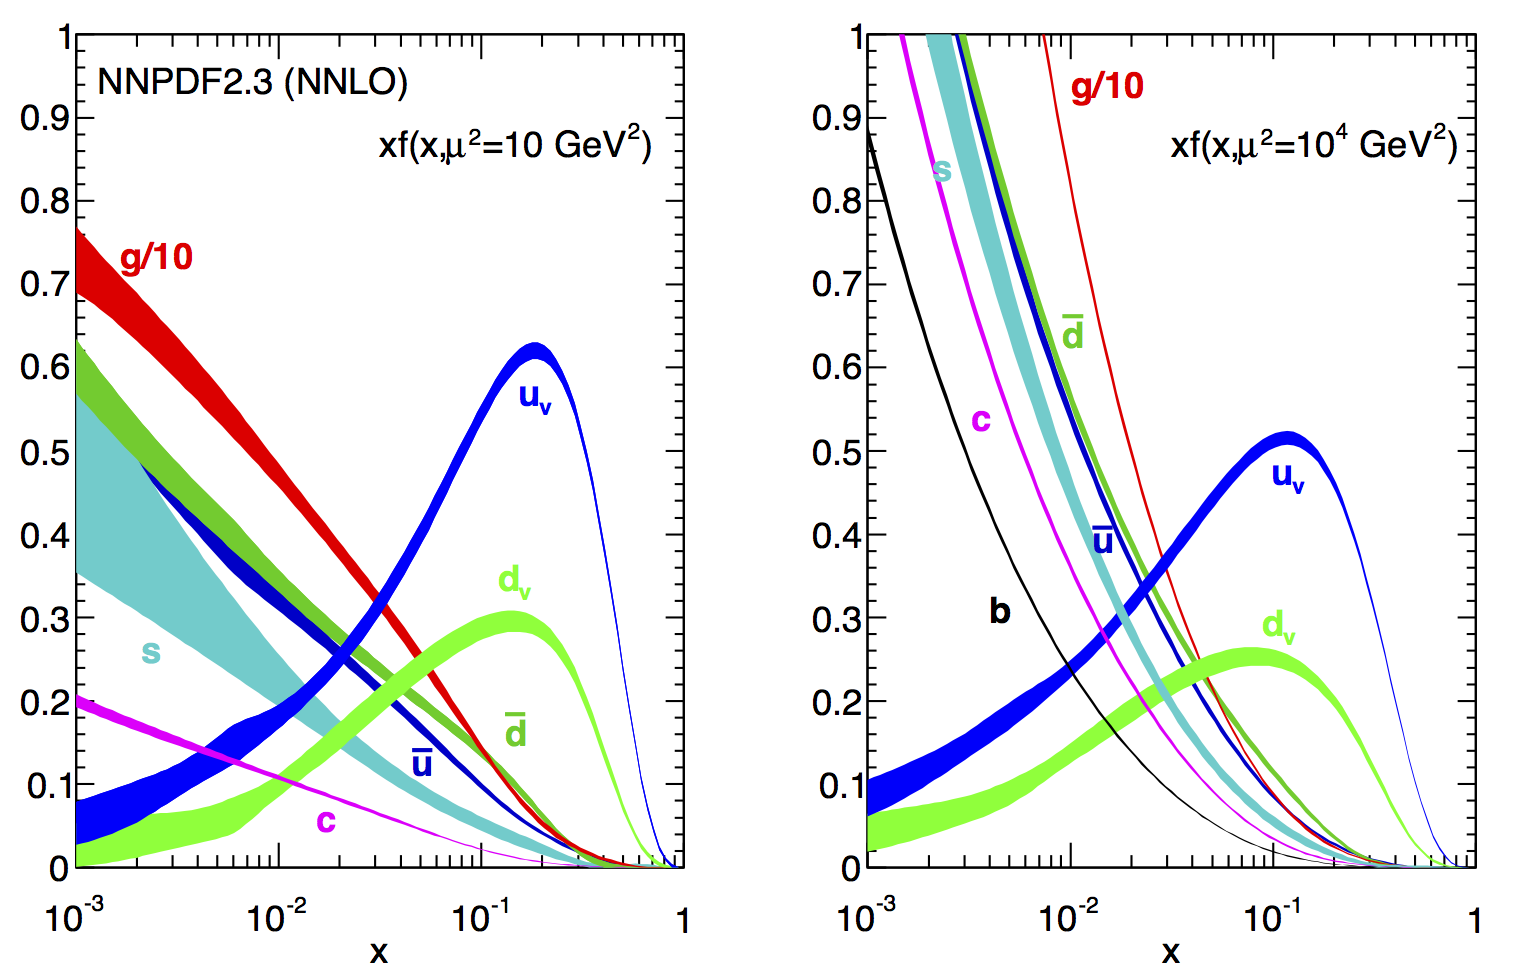
\includegraphics[width=0.75\textwidth]{figures/nnpdf23_nnlo_allpdfs.png}
\caption[Parton distribution functions of the NNPDF Collaboration]{Parton distribution functions of the the NNPDF Collaboration for two different energy scales~\cite{NNPDF23}. The x-axis denotes the momentum fraction $x$
carried by the valence quarks, the sea quarks and gluons.}
\label{figure_parton_distribution_functions}

\end{figure}
Collisions at LHC take place between two quarks, two gluons or a quark and a gluon. Therefore the real center-of-mass energy at each
collision, paying respect to the PDFs, is unknown. Since the partons of the proton are strongly interacting, QCD processes will play a huge role
for all hard-scattering processes, especially the search for the SM Higgs boson.

\section{The Higgs Mechanism and Its Consequences}
\subsection{EBH Mechanism and the Higgs boson}


As already mentioned before, the SM is lacking mass terms in the lagrangian. In order to keep the SM lagrangian renormalizable one has
to demand gauge invariance. Artificially introducing mass terms to the SM lagrangian violates this fundamental principle. Therefore
a new mechanism has to be introduced by which the weak gauge bosons gain their mass.

A new scalar field $\scalarField$ is introduced. This scalar doublet reads: \\
\begin{gather}
\scalarField =  \begin{pmatrix} \phi^+ \\ \phi^0 \end{pmatrix} = \frac{1}{\sqrt{2}} \begin{pmatrix}  \phi_1 + i \phi_2 \\ \phi_3 + i \phi_4\end{pmatrix}
\end{gather}
A lagrangian based on this field can be constructed, containing a term for the kinetic energy and one for the potential energy.
\begin{gather}
    \label{eq_lagrangian_higgs}
    \mathcal{L}_\mathrm{Higgs} = \underbrace{(\mathrm{D}\xspace^\mu \, \Phi)^\dagger (\mathrm{D}\xspace_\mu \, \Phi)}_{\text{Kinetic}} \underbrace{- \mu^2 \, \Phi^\dagger \, \Phi - \lambda {(\Phi^\dagger \, \Phi})^2}_{\text{Potential}}
\end{gather}

The potential contains two parameters: $\lambda$ and $\mu^2$. The first parameter is real and positive and
describes a self coupling term. The other term, containing $\mu^2$, looks already like a mass-type term.
If $\mu^2$ is chosen to be positive, there is only one ground state possible: $\av{\Phi}_{min}=0$. But this will not solve the
aforementioned mass problem. Choosing $\mu^2$ to be negative leads to the following minimum of the potential: \\
\begin{gather}
\frac{\partial V}{\partial \Phi^\dagger \Phi} = \mu^2 +2 \lambda \Phi^\dagger \Phi \\
\Rightarrow \abs{\Phi_{min}} = \sqrt{\frac{-\mu^2}{2\lambda}} = \frac{v}{\sqrt{2}},
\end{gather}
where $v$ denotes the vacuum expectation value (\VEV). Without the loss of generality the fields $\Phi_i, i=1..4$ can be chosen in the following way:
\begin{gather}
\Phi_1= \Phi_2 = \Phi_4 = 0 \quad \text{and} \quad \Phi_3 = \Phi_{min}
\end{gather}
Now the ground state of the potential is no longer symmteric under $\mathrm{SU}(2)$ rotations, but still keeping the renormalizability, which was shown in 1972~\cite{THOOFT1972189}.
This choice leads to a ground state which can be expanded by using the Higgs field $h(x)$:
\begin{gather}
    \av{\Phi}_0 = \frac{1}{\sqrt 2} \, \begin{pmatrix} 0 \\ v \end{pmatrix} \quad \Rightarrow \quad \Phi(x) = \frac{1}{\sqrt 2} \, \begin{pmatrix} 0 \\ v + h(x) \end{pmatrix}
\end{gather}
With $\Phi(x)$ one can expand $\mathcal{L}_\mathrm{Higgs}$~\ref{eq_lagrangian_higgs}. The kinetic term $\abs{\mathrm{D}\xspace_\mu \, \Phi}^2$ reads:
\begin{align}
    %\abs{\covdif_\mu \, \Phi}^2 = \frac 1 2 \del{\partial_\mu \, H}^2 + \frac 1 8 \, g_2^2 \del{v+H}^2 \, \abs{W_\mu^1 + \im \, W_\mu^2}^2 + \frac 1 8 \del{v+H}^2 \, \abs{g_2 \, W_\mu^3 - g_1 \, B_\mu}^2
    \abs{\mathrm{D}\xspace_\mu \, \Phi}^2 &= \frac 1 8 \, v^2 \, g_2^2 \, \abs{W_\mu^1 + \im \, W_\mu^2}^2 + \frac 1 8 \, v^2 \, \abs{g_2 \, W_\mu^3 - g_1 \, B_\mu}^2 + \, \ldots \\
    &= \frac 1 2 \, m_W^2 \, W_\mu^+ \, W^{- \mu} + \frac 1 2 \, m_Z^2 \, Z_\mu \, Z^\mu + 0 \cdot A_\mu A^\mu\
\end{align}
Here $v$ denotes the \VEV, $g$ the coupling constant and $W^{1,2,3}_{\mu}$ and $B_{\mu}$ the gauge fields of the electroweak theory.
$W^\pm_{\mu}, Z_{\mu}$ and $A_{\mu}$ are the physical representations of these gauge fields.
Finally one can see that the kinetic term directly rises mass terms for the weak gauge bosons, but not for the photon.
The same expansion can be done for the potential of the Higgs lagrangian:
\begin{gather}
    V = \frac 1 2 \, \mu^2 \, (v+H)^2 + \frac 1 4 \, \lambda (v+H)^4 \quad \Rightarrow \quad m_H = -\sqrt 2 \, \mu = v \, \sqrt{2 \, \lambda}
\end{gather}
A very interesting property of the Higgs field appears: It comes along with a new particle with the mass $m_H =v \, \sqrt{2 \, \lambda}$, the SM Higgs boson.
Additionally one can see trilinear and quartic self-coupling terms in the expansion of the potential.

All in all a mechanism is introduced, which spontaneously breaks the $\mathrm{SU}(2)$ symmetry, but not the $\mathrm{U}(1)$ or $\mathrm{SU}(3)$ symmetry.
This leads to mass terms for the weak gauge bosons, but not for the photon or the gluon, while keeping the SM lagrangian renormalizable.

\subsection{Yukawa Interaction}

In order to generate mass to the fermions, using the same principle as before, Yukawa interaction terms are added to the lagrangian.
Yukawa interaction describes the interaction between a scalar field (Higgs field) and a Dirac field (fermion field).
Additionally one has to pay respect to the chirality of the fermions. The lagrangian for the fermion mass then reads:
\begin{gather}
    \label{eq_lagrandian_mf}
    \mathcal{L}_\mathrm{m_f}= - \lambda_f \, (\ensuremath{\psi}\xspace_\mathrm{L}^\dagger \, \Phi \, \ensuremath{\psi}\xspace_\mathrm{R}+ \ensuremath{\psi}\xspace_\mathrm{R}^\dagger \, \Phi^\dagger \, \ensuremath{\psi}\xspace_\mathrm{L}) \quad \text{with} \quad \Phi(x) = \frac{1}{\sqrt 2} \, \begin{pmatrix} 0 \\ v + H(x) \end{pmatrix}
\end{gather}
Here $\ensuremath{\psi}\xspace_\mathrm{L}$ describes the left-handed doublet and $\ensuremath{\psi}\xspace_\mathrm{R}$ the right-handed singlet.
After spontaneous symmetry breaking the fermion mass $m_f$ and the coupling to the Higgs field $g_{Hff}$ appear:
\begin{gather}
m_f = \frac{v}{2} \, \lambda_f \inote{and} g_{Hff} = \frac{m_f}{v}
\end{gather}
This principle now also generates mass for the fermions. Finally one can conclude from the coupling to the Higgs field,
that the coupling strength is proportional to the fermion mass.

\subsection{Properties of the Higgs Boson}

The Higgs boson differs from all other fundamental particles, since it has spin 0. It also is electrically neutral and does
not carry any color charge. Its CP eigenvalue is predicted to be +1 and the only eigenvalue of the Higgs boson, which is
not measured up to now.

In the past ~50 years two accelerators were built with the main goal to find the Higgs boson. The first was the \LEP accelerator,
which was a electron-positron collider. Unfortunately it was not able to discover the Higgs boson, but strong exclusion limits
could be set. Afterwards the \LHC was built using the \LEP tunnel. The \LHC is a proton-proton collider running on high
center-of-mass energies, which makes it a "discovery machine" and able to finally discover the Higgs boson. The relevant Higgs production
feynman diagrams for such a machine are shown in figure~\ref{figure_higgs_production_feynman}.\\

\begin{figure}[h!]
\centering
\subfloat[ggF]{ \label{figure_higgs_production_feynman_gluon_fusion}
	\centering \begin{tikzpicture}[line width=1.5pt, scale=1.2]
\draw[step=0.5cm, very thin, transparent] (0cm,0cm) grid (4cm,2cm);

\draw[gluon, lightgray] (0.5cm,0cm+0.15cm) -- (1cm,1.25cm);
\draw[gluon, lightgray] (1.5cm+0.7cm,1cm+1cm-0.7cm) -- (3.25cm,2cm);

\draw[gluon] (0cm,0cm) -- (1.5cm,0cm);
\node at (0cm-0.2cm,0cm) {g};

\draw[gluon] (0cm,2cm) -- (1.5cm,2cm);
\node at (0cm-0.2cm,2cm) {g};

\draw[scalarnoarrow, color1, line width=3pt] (2.5cm,1cm) -- (4cm,1cm);
\node at (4cm+0.3cm,1cm) [color1]{H};

\draw[fermion] (2.5cm,1cm) -- (1.5cm,0cm);
\draw[fermion] (1.5cm,2cm) -- (2.5cm,1cm);
\draw[fermion] (1.5cm,0cm) -- node[right]{t} (1.5cm,2cm);
\end{tikzpicture}

}
\hspace{0.05\textwidth}
\subfloat[VBF]{ \label{figure_higgs_production_feynman_vector_boson_fusion}
	\centering \begin{tikzpicture}[line width=1.5pt, scale=1.2]
\draw[step=0.5cm, very thin, transparent] (0cm,0cm) grid (4cm,2cm);

\draw[fermion] (0cm,0cm) -- (2cm,0cm);
\node at (0cm-0.3cm,0cm) {$q_2$};

\draw[fermion] (2cm,0cm) -- (4cm,0cm);
\node at (4cm+0.3cm,0cm) {$q_2'$};

\draw[fermion] (0cm,2cm) -- (2cm,2cm);
\node at (0cm-0.3cm,2cm) {$q_1$};

\draw[fermion] (2cm,2cm) -- (4cm,2cm);
\node at (4cm+0.3cm,2cm) {$q_1'$};

\draw[scalarnoarrow, color1, line width=3pt] (2cm,1cm) -- (4cm,1cm);
\node at (4cm+0.3cm,1cm) [color1]{\PHiggs};

\draw[vector] (2cm,1cm) -- node[left]{$W$, $Z$} (2cm,0cm);
\draw[vector] (2cm,1cm) -- node[left]{$W$, $Z$} (2cm,2cm);
\end{tikzpicture}

}
\\ \vspace{5mm}
\subfloat[VH]{ \label{figure_higgs_production_feynman_higgs_strahlung}
	\centering \begin{tikzpicture}[line width=1.5pt, scale=1.2]
\draw[step=0.5cm, very thin, transparent] (0cm,0cm) grid (4cm,2cm);

\draw[fermionbar] (0cm,0cm) -- (1.25cm,1cm);
\node at (0cm-0.2cm,0cm) {$\overline{q}$};

\draw[fermion] (0cm,2cm) -- (1.25cm,1cm);
\node at (0cm-0.2cm,2cm) {$q$};

\draw[scalarnoarrow, color1, line width=3pt] (2.75cm,1cm) -- (4cm,2cm);
\node at (4cm+0.3cm,2cm) [color1]{\PHiggs};

\draw[vector] (2.75cm,1cm) -- node[below]{$W^*$, $Z^*$} (1.25cm,1cm);

\draw[vector] (2.75cm,1cm) -- (4cm,0cm);
\node at (4cm+0.4cm,0cm) {$W$, $Z$};
\end{tikzpicture}

}
\hspace{0.05\textwidth}
\subfloat[ttH]{ \label{figure_higgs_production_feynman_associated_production}
	\centering \begin{tikzpicture}[line width=1.5pt, scale=1.2]
\draw[step=0.5cm, very thin, transparent] (0cm,0cm) grid (4cm,2cm);

\draw[gluon] (0cm,0cm) -- (2cm,0cm);
\node at (0cm-0.2cm,0cm) {$g$};

\draw[gluon] (0cm,2cm) -- (2cm,2cm);
\node at (0cm-0.2cm,2cm) {$g$};

\draw[scalarnoarrow, color1, line width=3pt] (2cm,1cm) -- (4cm,1cm);
\node at (4cm+0.3cm,1cm) [color1]{\PHiggs};

\draw[fermion] (4cm,0cm) -- (2cm,0cm);
\node at (4cm+0.4cm,0cm) {$\overline{t}$};

\draw[fermion] (2cm,0cm) -- (2cm,1cm);
\draw[fermion] (2cm,1cm) -- (2cm,2cm);

\draw[fermion] (2cm,2cm) -- (4cm,2cm);
\node at (4cm+0.4cm,2cm) {$t$};
\end{tikzpicture}

}
\caption{Feynman diagrams of the four main Higgs production modes at \LHC.}
\label{figure_higgs_production_feynman}
\end{figure}

The gluon fusion process (ggF)~\ref{figure_higgs_production_feynman_gluon_fusion} is the most dominant production process at \LHC. Two gluons produce a top loop,
which couples to the Higgs boson. The loop can be produced by any quark, but it was shown before, that the fermion mass
is proportional to the coupling to the Higgs boson. This makes the heaviest fermion the most probable to participate in this loop:
the top quark. As shown in the feynman diagram jets can be radiated of the gluons or the loop causing a phenomena called
initial state radiation (ISR). The radiation of jets boosts the Higgs boson, which can be exploited in Higgs searches, but also reduces
the cross section of this Higgs production.

The second most prominent process is vector boson fusion (VBF)~\ref{figure_higgs_production_feynman_vector_boson_fusion}.
Two quarks radiate weak gauge bosons, which annihilate and produce a Higgs boson. The two quarks are then scattered into opposite
directions, leading to a very clear detector signature of two forward jets.

The Higgs strahlung process (VH)~\ref{figure_higgs_production_feynman_higgs_strahlung} is suppressed at \LHC since it requires the
annihilation of two quarks. This process would be the most dominant at a proton-antiproton collider, such as \Tevatron at \Fermilab.
The annihilation produces an excited $\PW^*$ or $\PZ^*$ boson, which deexictes by radiating a Higgs boson.

The last remaining process it the top associated Higgs production (ttH)~\ref{figure_higgs_production_feynman_associated_production}.
This process is highly suppressed, since it requires energies to produce two top quarks and a Higgs boson in the final state. It is
neglected in most analysis.

Figure~\ref{figure_higgs_production_cross_sections} shows the cross sections for the different Higgs productions and their total uncertainties
at the \LHC for two different center-of-mass energies as a function of the Higgs boson mass $m_H$.


\begin{figure}[h]
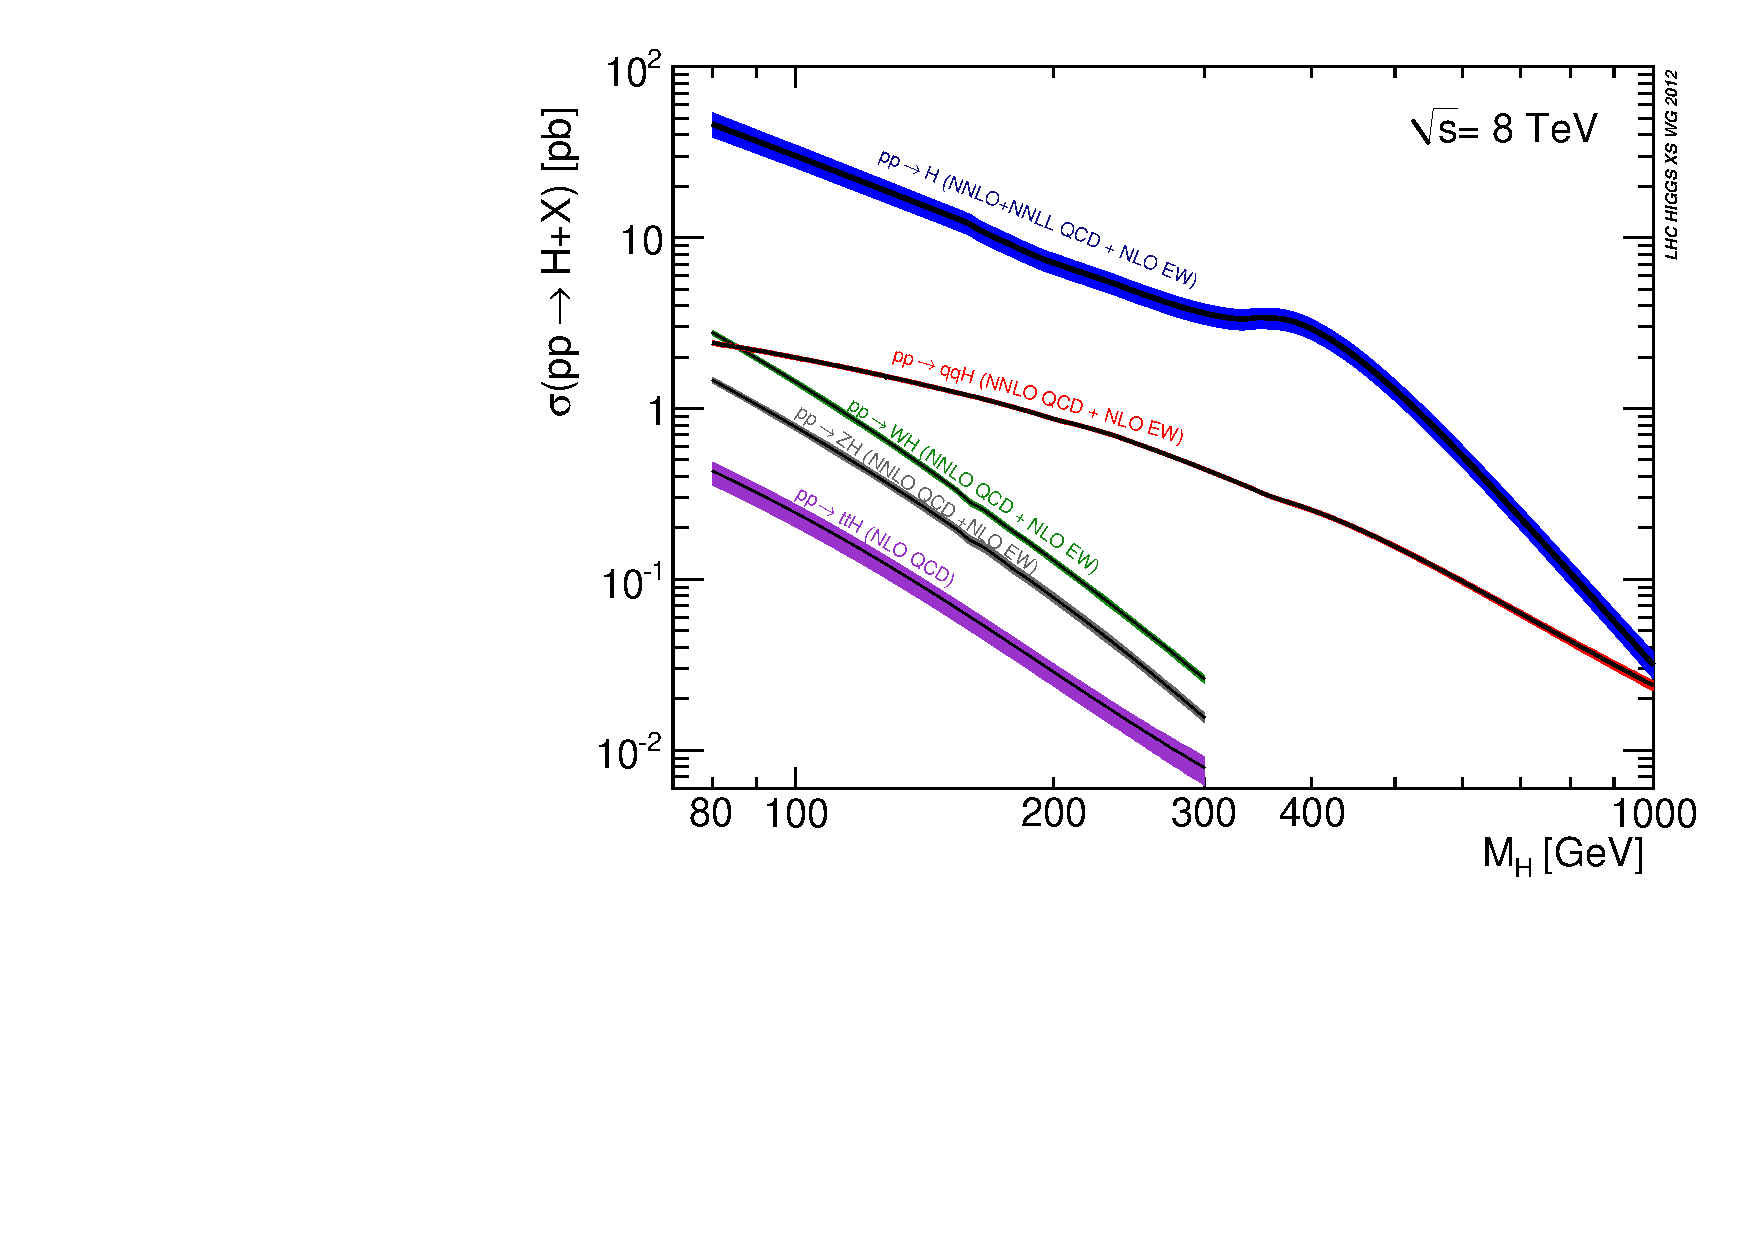
\includegraphics[width=0.48\textwidth]{figures/Higgs_XS_8TeV_lx.pdf}
\hfill
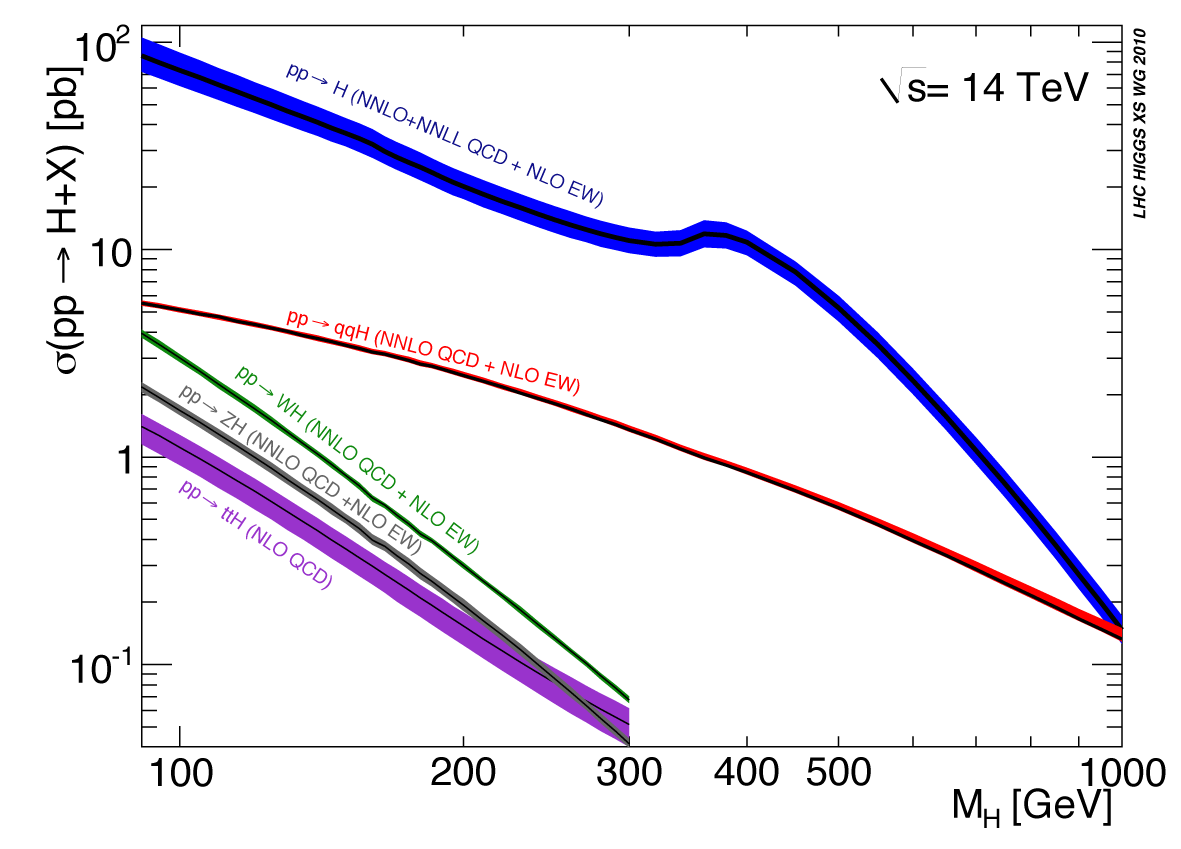
\includegraphics[width=0.48\textwidth]{figures/YRHXS_Summary_fig3}
\caption[Higgs boson production cross sections.]{Predicted Higgs boson production cross sections for center-of-mass energies of $\sqrt s=\unit{8}{\TeV}$~(left) and \unit{14}{\TeV}~(right)~\cite{yellow_report_1, yellow_report_2, yellow_report_3}.}
\label{figure_higgs_production_cross_sections}
\end{figure}
